\chapter{Introduction}

The Standard Model (SM) of particle physics is one of the most successful and precise theories developed in physics as it can describe observed phenomena over a large energy range (\cite{omg}, \cite{hydrogen}) with high precision~\cite{mu}. The theoretical foundations could only be developed and tested by the accurate measurements performed at particle physics experiments all over the world. One of these experiments was the Belle experiment in Tsukuba, Japan, which was used to measure parameters of the SM with high precision. 

However, there are many experiments which indicate that the SM is not the definite theory for particle physics. One example is the observation of rotational velocities of galaxies \cite{galaxy} which can be explained by introducing the invisible ``dark matter''. Not much is known about this new type of matter which is not part of the SM -- especially not its interactions with other particles or its characteristics like mass or spin. Another example is the imbalance between the observed matter and antimatter in the universe, which can be described by baryon number violation, C and CP violation and thermodynamic inequalities in the early universe~\cite{sakharov}. Although there is theoretically well-understood CP violation in the SM~\cite{CP_theory}, which was observed at the Belle experiment~\cite{CP}, this CP violation can not sufficiently create a matter--antimatter asymmetry of the measured size. Additionally, there are many candidates for new models beyond the SM like Supersymmetry~\cite{susy}, which can answer open questions of the SM. Those theories introduce new particles that can be observed indirectly by their impact on the interactions between the SM particles if these interactions are measured precisely enough.

Therefore the successor of Belle -- Belle~II -- was planed and is currently being constructed to replace most of the Belle detector~\cite{tdr}. It is built with advanced measuring devices and will be used to record a larger number of $\PB$ mesons -- the successor of the $\Pep\Pem$-collider (SuperKEKB) is planed to have an instantaneous luminosity 40 times higher than that of KEKB. The produced $\PB$ mesons decay and by measuring the characteristics of the decay products like their momentum and their type one can draw conclusions on the primary, high energetic process.

% \begin{center}
%   \centering
%   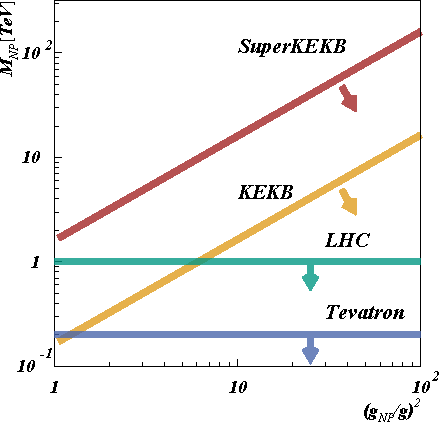
\includegraphics[width=0.6\linewidth]{figures/general/luminosity.pdf}
% \end{center}

One of the key elements for measuring the decay products in the Belle~II experiment are the tracking detectors~\cite{tdr}. Their function is to detect the produced particles as well as to quantify their trajectory parameters, e.g.\ their momentum. To serve this purpose, space-resolved measuring devices in a homogeneous magnetic field are used to detect the locations of points on the curled trace of the charged particles through the detector, so-called hits. As there is no way to obtain information on which particle has produced which hit, this decision has to be made by algorithms implemented mainly in offline software. These algorithms are called track finders and work with procedures comparable to pattern recognition tasks as they use the typical shape of the tracks in the detector to partition the hits. Their output is an exclusive sets of hits which were possibly created by the same particle. The next step -- the track fitter~\cite{genfit} -- determines the parameters of the trajectories.

As the tracking detectors are the only detector part with the task to find and measure all charged decay products, it is very important to find as many tracks as possible. High energy losses of the particles or multiple scattering in the detector elements can lead to deviations from the typical circular-shaped trajectory which can decrease the finding efficiency. Imperfections in the software and hits produced by beam-induced background (e.g.\ via secondary photon showers originating from scattered electrons or positrons), which is enhanced because of the higher luminosity of SuperKEKB, can lead to wrongly added hits or tracks and can deteriorate the resolution of the trajectory parameters calculated while fitting. To reach the performance of the track finders for the Belle experiment despite the higher background, the tracking software was rewritten with newly developed or refined algorithms.

Studies of rare decays use typically only a small number of events~\cite{lutz} to perform their measurements, so loosing events because of a reduced finding efficiency can lead to crucial problems in these channels or could make it even impossible to search for these decays. Also high-statistic studies performed with millions of events can be improved by a better tracking software, as the trajectory parameters go directly into the variables needed in the analyses and smaller errors on these parameters can improve the overall systematic uncertainty. As some analyses depend on the fact, that the whole event with all its measurements can be described consistently by a given model (by using variables as the measured energy still left in the detector after subtracting all reconstructed and classified particles~\cite{christian_phd}), the finding efficiency of the tracks together with a high purity plays a crucial role.

After an introduction into relevant parts of the Belle~II detector in chapter~\ref{chapter-ex}, the algorithms behind the track finders as well as the calculated figures of merit will be described (chapter~\ref{chapter-theory}). The main part of this thesis will be dedicated to the improvements on the tracking software for the central drift chamber (CDC) -- the largest tracking detector of Belle~II. In chapter~\ref{chapter-workflow}, the newly developed algorithms together with their implementation will be described and evaluated. Among these algorithms is the hit finder for stereo hits, which are hits originating from sense wires with a small tilting angle that make it possible to determine the trajectory along the beam direction. Compared to the old implementation, the results have been improved significantly while also lowering the computing time drastically.

This thesis was the first to combine all developed CDC track finding algorithms implemented for Belle~II, so a description of their characteristics and the algorithms for their combination will also be discussed in this chapter. The implemented changes increased the number of correctly found tracks and hits. Additionally, the number of wrong tracks and also the computing time of the whole algorithm was decreased. The track finders were enhanced to outperform the reference implementation copied from the former Belle experiment for the first time in figures of merit as well as computing performance and therefore the transition from this reference implementation to the newly developed track finders was made.
\clearpage
Pions with low momenta in the region of $\unit[50]{MeV} - \unit[100]{MeV}$ play an important role for many planned physics analyses. Because of their low momentum, they can not reach the CDC and can only be detected in the inner most detectors -- the vertex detectors (VXD). This however decreases their momentum resolution because of a smaller lever arm. To increase this resolution -- which is very important for the physics analyses -- again, another piece of information apart of the location of hits in the vertex detector is used: the energy loss per travel length. This value is connected to the momentum by the Bethe equation and can be used as input to the fitting routine~\cite{robert}. The newly developed procedure in this thesis to use the momentum estimation of every hit separately, which could increase the number of successful fits as well as the momentum resolution drastically in the region $\unit[50]{MeV} - \unit[80]{MeV}$, will be described in chapter~\ref{chapter-vxd}.

